\chapter{Étude du protocal de bi-partition : Mesure de distribution de rapidités locales $\rho(x , \theta ) $  pour des systèmes hors équilibre}
\minitoc


\section*{Introduction}


\paragraph{Objectif de ce chapitre :}
Ce chapitre est consacré à l’étude de la dynamique hors équilibre d’un gaz quantique unidimensionnel intégrable, soumis à une discontinuité initiale de densité induite par un protocole de type {\bf quench bipartite}. L’objectif principal est d’évaluer dans quelle mesure la Théorie Hydrodynamique Généralisée (GHD) permet de décrire cette dynamique, tant sur le plan théorique qu’expérimental. Nous nous appuyons sur une préparation initiale contrôlée, un protocole de coupure abrupte, et une analyse des profils de densité et des facteurs d’occupation pour tester les prédictions de la GHD.

\paragraph{Modèles intégrables et thermalisation généralisée :}
Les modèles intégrables jouent un rôle central dans l’étude des systèmes quantiques à plusieurs corps, notamment en régime hors équilibre. Leur caractéristique essentielle est la présence d’une infinité de constantes du mouvement, qui empêche l’évolution vers l’équilibre thermodynamique canonique. Cette contrainte mène à l’émergence d’un état d’équilibre généralisé, décrit non par l’ensemble canonique, mais par l’{\bf Ensemble de Gibbs Général (GGE)}\index{Ensemble Thermodynamique Général (GGE)}\index[pers]{Ensemble Thermodynamique Général (GGE), Ensemble de Gibbs Général (GGE)}, qui maximise l’entropie sous contraintes intégrales multiples (cf Chap (\ref{chap:relaxation})).

\paragraph{Une analogie classique : le pendule de Newton :}
Une illustration classique du comportement non diffusif des systèmes intégrables est fournie par le pendule de Newton : les chocs élastiques entre sphères de masses égales conduisent à une propagation balistique de l’énergie, sans diffusion. Cette analogie, bien que classique, capture l’essence du transport cohérent que l’on retrouve dans les systèmes intégrables quantiques.

\paragraph{Le problème de Riemann en hydrodynamique :}
Un test fondamental de la dynamique hors équilibre est fourni par le problème dit de Riemann, qui consiste à étudier l’évolution d’un système à partir d'une discontinuité initiale dans l'espace. Dans sa formulation générale, on considère une équation de conservation de la forme
\begin{eqnarray}\label{chap6:eq.Rieman.1}
\partial_t u + \partial_x f(u) = 0,
\end{eqnarray}
accompagnée d'une condition initiale arbitraire $u(x, t = 0) = u_0(x)$.
Dans le cas particulier que nous considérons ici, l’état initial est composé de deux régions homogènes, juxtaposées de part et d’autre de l’origine :
\begin{eqnarray}\label{chap6:eq.Rieman.cond.1}
	u( x, t=0 ) = \left \{\begin{array}{rcl} u_g & \text{si} & x<0 \\ u_d & \text{si} & x > 0 \end{array} \right. \,.
\end{eqnarray}
Ce type de configuration, appelé problème de Riemann à données discontinues, permet de sonder la réponse non linéaire du système.
%Sa résolution dans des systèmes intégrables, notamment en présence de degrés de liberté internes ou d’interactions fortes, est longtemps restée une question ouverte.

\paragraph{Le problème de Riemann quantique : un cadre paradigmatique.}

Dans un système quantique intégrable, le problème de Riemann consiste à connecter brusquement deux régions préparées dans des états thermodynamiques différents, généralement homogènes. Ce scénario, dit de \emph{quench bipartite}, constitue un cadre paradigmatique pour sonder la dynamique hors équilibre dans les gaz quantiques unidimensionnels~\cite{doyon2017lecture,bertini2016transport}. Contrairement au cas classique, la présence d’un nombre infini de constantes du mouvement empêche l’établissement d’un état thermique usuel. La relaxation locale conduit alors à un état d’équilibre généralisé, spécifique à chaque région de l’espace-temps. Le problème de Riemann quantique permet ainsi d’étudier la propagation balistique d’informations, l’émergence d’un régime autosimilaire stationnaire, et la structure fine des distributions locales de quasi-particules. Il offre un terrain théorique idéal pour tester la validité de la Théorie Hydrodynamique Généralisée~\cite{castro2016emergent,doyon2017ghd}, tout en étant expérimentalement accessible grâce aux systèmes ultrafroids unidimensionnels.

\paragraph{Apparition de la Théorie Hydrodynamique Généralisée (GHD) :}
L’avènement de la GHD a marqué une avancée majeure dans la compréhension de la dynamique des systèmes intégrables. Introduite dans le contexte des théories des champs (modèle de Sinh-Gordon, modèle de Lieb-Liniger) et des chaînes quantiques (chaîne XXZ de Heisenberg) [références à insérer], elle permet de décrire analytiquement la propagation d’informations dans ces systèmes en intégrant les contraintes des charges conservées. Plusieurs solutions analytiques du problème de Riemann ont depuis été obtenues, notamment dans la chaîne XXZ et pour des gaz de sphères dures en 1D, confirmant la validité et la puissance prédictive de la GHD.

\paragraph{Notre système : un gaz de bosons 1D faiblement interactifs :}
Nous considérons un gaz quantique unidimensionnel de bosons faiblement interactifs, confiné dans une géométrie strictement 1D, et bien décrit par le modèle intégrable de Lieb-Liniger avec interactions répulsives. Ce système présente un comportement quantique collectif tout en restant dans un régime faiblement corrélé, ce qui en fait un candidat idéal pour tester les prédictions de la GHD.

\paragraph{Préparation expérimentale et protocole de coupure :}
La configuration initiale consiste à préparer un gaz homogène à densité constante $n_0$, et à température contrôlée (voir Fig.~\ref{fig:BiPart.insitut}). Un protocole de coupe abrupte est ensuite appliqué : la partie gauche du système ($x<0$) est vidée de ses atomes, tandis que la partie droite ($x>0$) reste occupée. Ce \emph{quench bipartite} génère une discontinuité initiale de densité, analogue au problème de Riemann, mais dans un système quantique doté d’un nombre infini de lois de conservation. Ce protocole a déjà fait l’objet d’une première étude expérimentale dans la thèse de Léa Dubois \cite{DuboisThese}, qui en a révélé le potentiel pour sonder la dynamique hors équilibre.

\paragraph{Observation d’une propagation balistique :}
Nous prolongeons cette étude en analysant la dynamique unitaire du gaz à l’aide des outils de la GHD. Nous montrons que la discontinuité initiale donne lieu à une propagation balistique, en bon accord avec la solution du problème de Riemann généralisé. Le profil de densité mesuré à différents temps révèle une frontière en déplacement linéaire, reproduite avec précision par les prédictions théoriques (voir Fig.~\ref{fig:BiPart.coupure1} (e)-(g)). Des écarts résiduels, attribuables à des effets thermiques et à des imperfections expérimentales, sont toutefois observés.

\paragraph{Reconstruction de la distribution de rapidité :}
Un aspect central de notre approche repose sur la reconstruction de la distribution initiale de rapidité à partir des profils de densité mesurés dans la région de transition. Cette démarche s’apparente à une forme de *thermométrie généralisée*, et permet d’inférer des informations fines sur les états locaux du système.

\paragraph{Accès expérimental au facteur d’occupation $\nu(x,\theta)$ :}
Nous développons également une méthode expérimentale originale permettant de mesurer localement le facteur d’occupation $\nu(x,\theta)$ dans la région de déformation. Cette quantité révèle une forte asymétrie : large et lisse du côté initialement occupé, abrupte et tronquée du côté initialement vide. Ce comportement reflète la nature hors équilibre du système, et s’accorde qualitativement avec les prédictions de la GHD, bien que la résolution spatiale expérimentale limite l’accès aux détails les plus fins.

\paragraph{Conclusion :}
Ce chapitre explore ainsi, à la fois théoriquement et expérimentalement, la dynamique d’un gaz intégrable soumis à une discontinuité initiale de densité. Il met en lumière la pertinence de la GHD pour décrire de telles dynamiques, et démontre la faisabilité d’outils d’analyse avancés comme la reconstruction de la distribution de rapidité ou la mesure locale du facteur d’occupation.


\section{Dynamique balistique d’un gaz 1D après une coupure bipartite}

\subsection*{Introduction}

Dans cette section, nous étudions la dynamique hors équilibre d’un gaz quantique unidimensionnel de bosons soumis à une coupure bipartite. Ce protocole expérimental permet de générer une discontinuité nette dans le profil de densité initial, menant à une évolution balistique non triviale.

L’objectif est double :

\begin{itemize}[label = $\bullet$]
	\item du point de vue expérimental, suivre en temps réel l’évolution du gaz et caractériser ses propriétés locales et globales ;
	\item du point de vue théorique, confronter ces observations aux prédictions de la Théorie Hydrodynamique Généralisée (GHD), qui fournit un cadre analytique pour décrire la relaxation de systèmes intégrables à grande échelle.
\end{itemize}

Cette étude constitue une illustration directe du problème de Riemann quantique, dans lequel un état initial composé de deux régions thermodynamiques différentes évolue selon une dynamique déterministe. Elle permet également d’accéder à des signatures locales de la distribution de quasi-particules (ou rapidités), jusque-là difficiles à sonder expérimentalement.

\medskip

Nous structurons cette section en quatre sous-parties :
\begin{itemize}[label = $\bullet$]
	\item Préparation et protocole expérimental : description du gaz unidimensionnel, du piège et de la méthode de coupure.
	\item Cadre théorique de la GHD : présentation des équations hydrodynamiques et de la solution auto-similaire du problème de Riemann.
	\item Confrontation avec les données expérimentales : validation de la structure auto-similaire et test de la théorie à température nulle.
\end{itemize}


\subsection{Préparation expérimentale et protocole de coupure}
\label{chap6:sec.propcol}

{\color{blue} 
Points clés :
\begin{itemize}
	\item Réalisation d’un gaz unidimensionnel de bosons dans un piège quartique plat.
	\item Méthode d’illumination sélective à l’aide d’un DMD pour créer une discontinuité initiale.
	\item Passage à un régime d’expansion libre unidimensionnelle après suppression du confinement longitudinal.
\end{itemize}
}


\paragraph{Contexte expérimental et références}
Les détails concernant l’imagerie, le piégeage et la sélection spatiale sont présentés de manière approfondie dans le {chapitre~(\ref{chap:disp.exp})}, ainsi que dans la thèse de Léa Dubois \cite{L.Dubois2024}. Dans cette sous-section, nous nous limitons aux éléments essentiels à la compréhension du protocole de coupure et de la dynamique qui en résulte.

\begin{figure}[!htb]
\centering

\includegraphics[width=0.5\linewidth , page = 2 ]{figures/06_Bipart/Shemas_2.pdf}
\caption{Schéma synthétique du dispositif expérimental : cycles d’illumination, intensités de courant, géométrie du piège, et évolution du profil longitudinal au cours du protocole de coupure.}
\label{fig:setup}
\end{figure}

\paragraph{Préparation d’un gaz unidimensionnel de bosons} 
Nous utilisons un gaz ultra-froid de $^{87}$Rb, piégé sur une puce atomique dans l’état hyperfin $|F=2,m_F=2\rangle$. Le confinement transverse est assuré par trois microfils parcourus par des courants RF, produisant un piège harmonique de fréquence $\omega_\perp/2\pi = 2{,}56$~kHz. Après évaporation, on obtient un gaz à température $T \approx 100$~nK, dans un régime 1D caractérisé par $\mu, k_B T \ll \hbar \omega_\perp$. Le couplage effectif en 1D est $g = 2 a_{3D} \hbar \omega_\perp$, avec $a_{3D} = 5{,}3$~nm.

\paragraph{Confinement longitudinal quartique}
Le confinement longitudinal est généré par quatre fils latéraux, dont les courants sont ajustés pour annuler les composantes linéaire, quadratique et cubique du potentiel. Il en résulte un confinement quartique $V(x) = a_4 x^4$, produisant un profil de densité quasi-plat sur environ $250~\mu$m. Cette homogénéité est cruciale pour l’étude des dynamiques balistiques et pour l’application de la GHD.

\paragraph{Coupure bipartite par sélection spatiale}
La bipartition initiale est réalisée en illuminant l’extrémité gauche du gaz par un faisceau quasi-résonant façonné par un DMD. Les atomes exposés sont expulsés du piège via pression de radiation. Cette méthode, développée dans \cite{PhysRevLett.133.113402}, permet de créer une discontinuité nette du profil de densité, entre une région vide ($x<0$) et une région remplie homogène ($x>0$). %La résolution spatiale est limitée par celle du système d’imagerie (quelques $\mu$m).

\paragraph{Évolution après coupure}
Une fois la coupure effectuée, le confinement longitudinal est supprimé tandis que le confinement transverse est maintenu. Le gaz évolue alors librement dans une direction, ce qui est analogue au problème de Riemann \eqref{chap6:eq.Rieman.1} mais depuis une condition initiale de deux regions homogène \eqref{chap6:eq.Rieman.cond.1} . L’évolution du profil de densité $n(x,t)$ est suivie par imagerie après différentes durées $t$ d’évolution.

\begin{center}
	[figure de shemat de coupure en tikz zt au coter deux nuage , un coupé et l'autre non coupé]	
\end{center}

%\begin{figure}[!htb]
%\centering
%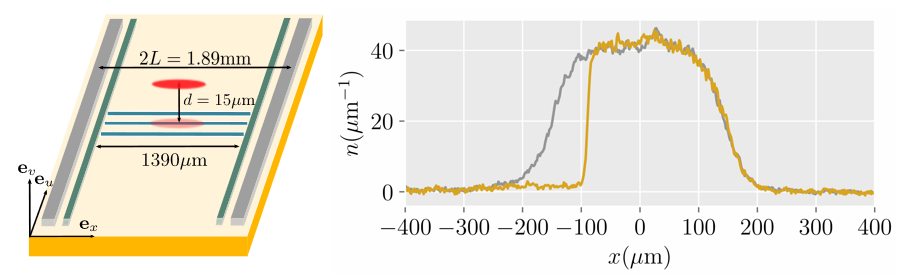
\includegraphics[width=0.9\linewidth]{figures/06_Bipart/Atom_chip.png}
%\caption{(a) Géométrie de la puce atomique. (b) Profils de densité longitudinale : en gris, gaz initial confiné dans un potentiel quartique ; en jaune, après illumination sélective et $1$~ms d’expansion libre.}
%\label{fig:setup}
%\end{figure}




\subsection{Cadre de la GHD et dynamique balistique et }
\label{sec.GHDpredictions}\label{sec:ghd}\label{chap6:sec:ghd}

{\color{blue}
Points clés :
\begin{itemize}
	\item Présentation du facteur d’occupation $\nu(x,\theta;t)$ comme variable hydrodynamique.
	\item Formulation de l’équation convective de GHD.
	\item Structure auto-similaire $\nu(x,\theta;t) = \nu^*(x/t,\theta)$ et résolution implicite via la vitesse effective.
	\item Prédictions analytiques pour le profil de densité $n(x,t)$.
\end{itemize}
}


Dans cette section, nous présentons le cadre théorique de la \emph{Théorie Hydrodynamique Généralisée} (GHD) appliqué à l’expérience décrite précédemment. L’objectif est de décrire analytiquement la dynamique balistique induite par une coupure bipartite dans un gaz quantique unidimensionnel, en exploitant les équations de GHD appliquées au modèle de Lieb-Liniger.\\

{\color{blue}
Nous procédons en plusieurs étapes : 
\begin{enumerate}
  \item Nous introduisons la description hydrodynamique à l’échelle d’Euler.
  \item Nous formulons les équations de GHD pour l’évolution du facteur d’occupation $\nu(x,\theta;t)$.
  \item Nous analysons la structure auto-similaire de la solution en régime hydrodynamique.
  \item Nous présentons la solution semi-analytique du problème de Riemann bipartite, ainsi que sa résolution graphique.
\end{enumerate}
}

\paragraph{Description hydrodynamique à l’échelle d’Euler}

Dans un système intégrable, les états stationnaires sont entièrement caractérisés par leur distribution de rapidités $\rho(\theta)$ ou, de manière équivalente, par le facteur d’occupation $\nu(\theta)$ (Cf {Chap~(\ref{chap:GHD})}). En régime hors équilibre, on suppose qu’à des échelles de temps longues et d’espace macroscopiques, le système évolue lentement vers un état localement stationnaire. Cela permet d’introduire une description hydrodynamique dans laquelle les quantités locales dépendent de la position et du temps : $\rho(x,\theta;t)$ ou $\nu(x,\theta;t)$.

%La densité linéique atomique est obtenue à partir de la distribution de rapidités par :
%\begin{equation}
%    n(x;t) = \int d\theta \, \rho(x,\theta ; t).
%    \label{eq:lineardensity}
%\end{equation}

\paragraph{Pourquoi travailler avec $\nu$ plutôt qu’avec $\rho$~?}
\subparagraph{Équation de GHD en termes de $\rho$.}
L’évolution à grande échelle du système est gouvernée par les équations de GHD~\cite{bertini_transport_2016, castro-alvaredo_emergent_2016}. 
L'évolution pour la distribution de quasi-particules $\rho(x,\theta;t)$ (Eq~\eqref{???}), en l'absence de potentiel extérieur, prend la forme d’une équation convective :
\begin{equation}
	\label{eq:rho.cont}
	\partial_t \rho + \partial_x \big( v^{\rm eff}_{[\rho]} \rho \big) = 0,
\end{equation}
où $v^{\rm eff}_{[\rho]}(\theta)$ est la vitesse effective des quasi-particules de rapidité $\theta$, fonctionnelle non linéaire de $\rho$ et où un terme de compression $\partial_x (v^{\rm eff}_{[\rho]} \rho)$ apparaît lorsqu’on développe la dérivée. Cela complique l’analyse, notamment lorsque les vitesses effectives varient fortement dans l’espace ou le temps.

Pour chaque rapidité $\theta$, l'équation \eqref{eq:rho.cont} constitue un cas particulier du problème de Riemann généralisé~\eqref{chap6:eq.Rieman.1}.
Nous considérons ici une condition initiale de type « coupure bipartite », représentant un état homogène à droite ($x>0$) et vide à gauche ($x<0$) :
\begin{equation}
    \label{eq:rho.cont.init}
    \rho(x,\theta;t=0) = 
    \begin{cases}
        \rho_0(\theta) & \text{si } x > 0, \\
        0 & \text{si } x < 0.
    \end{cases}
\end{equation}
Ce type de condition correspond , pour chaque rapidité $\theta$ , au condition introduit dans l'introduction \eqref{chap6:eq.Rieman.cond.1}.\\

\subparagraph{Équation de GHD en termes de $\nu$.}
En comparaison, l’évolution de la densité de remplissage $\nu(x,\theta;t)$ (Eq~\eqref{???}) , qui, en l’absence de potentiel extérieur suit une équation de transport pur (type Liouville) :
\begin{equation}
    \label{eq:nu.cont}
    \partial_t \nu + v^{\rm eff}_{[\nu]} \, \partial_x \nu = 0,
\end{equation}
où la dérivée temporelle est directement couplée à une dérivée spatiale. Cette forme préserve l'information le long des caractéristiques associées aux vitesses effectives $v^{\rm eff}_{[\nu]}$, ce qui rend la dynamique plus lisible et plus simple à analyser.

Les équation de transport pur \eqref{eq:nu.cont} ne sont pas  des cas particuliers du problème de Riemann généralisé~\eqref{chap6:eq.Rieman.1}. Et donc même si les conditions initials de type  « coupure bipartite » , pour $\nu$ :
\begin{equation}
    \label{eq:nu.cont.init}
    \nu(x,\theta;t=0) = 
    \begin{cases}
        \nu_0(\theta) & \text{si } x > 0, \\
        0 & \text{si } x < 0.
    \end{cases}
\end{equation}
sont du type \eqref{chap6:eq.Rieman.cond.1}, contrairement à \eqref{eq:rho.cont}, l'evolution \eqref{eq:nu.cont} ne génère pas de {\bf chocs}.\\


Dans ce travail, nous choisissons de formuler la dynamique hydrodynamique généralisée en termes de la fonction d’occupation $\nu(x,\theta;t)$, plutôt que de la densité de quasi-particules $\rho(x,\theta,t)$. Cette approche présente plusieurs avantages. D’une part, l’équation vérifiée par $\nu$ est une équation de transport pur \eqref{eq:nu.cont}, ce qui permet une résolution naturelle par la méthode des caractéristiques, plus simplement que dans \eqref{eq:rho.cont}. D’autre part, $\nu$ possède une interprétation physique claire comme taux de remplissage des états accessibles, borné entre 0 et 1, ce qui en fait une variable plus stable et mieux adaptée aux calculs analytiques ou numériques.
De plus, la dynamique effective des observables s’exprime naturellement en fonction de $\nu$.
Enfin, $\nu$ et $\rho$ étant liés, résoudre l’équation en $\nu$ revient, une fois $v^{\rm eff}_{[\nu]}$ déterminé, à résoudre complètement la dynamique de $\rho$.

\paragraph{Structure auto-similaire de la solution}
Un point central est que les conditions initiales ~\eqref{eq:nu.cont.init} sont invariantes par dilatation. En effet quelque soit $\alpha >0$ , et pour tout $x$ réelle, on a $\nu(\alpha x , \theta ; t = 0 ) = \nu( x , \theta ; t = 0 ) $.
Un autre point central de la GHD est l’invariance d’échelle des solutions de l’équation~\eqref{eq:nu.cont} ( \eqref{eq:rho.cont} aussi et plus généralement de \eqref{chap6:eq.Rieman.1}) . En effet, si $\nu(x,\theta;t)$ est solution de  l’équation~\eqref{eq:nu.cont}, alors $\nu(\alpha x, \theta; \alpha t)$ l’est également ,  pour tout $\alpha > 0$ , avec les conditions initiales $\nu(\alpha x , \theta ; t = 0 )$. {\color{blue} Comme les fonctions $\nu(\alpha \cdot , \theta ; t = 0 )$ et $\nu( x , \theta ; t = 0 )$ coïncident, alors si $\eqref{eq:nu.cont}$ admet au plus une solution physique ( entropique Cf Annex ~\ref{chap6:annex.Rieman}) pour chaque données initiales, on doit avoir $\nu( \alpha x , \theta ; \alpha t ) = \nu(  x , \theta ;  t )$ pour tout $\alpha > 0 $}. Sous hypothèse d’unicité (Cf Annex ~(\ref{chap6:annex.Rieman})), cette propriété implique que :
\begin{equation}
    \nu(x,\theta;t) = \nu^*\left(\frac{x}{t},\theta\right),
    \label{eq:nuvsnuetoile}
\end{equation}
autrement dit, les solutions dépendent uniquement du rapport $\xi = x/t$, appelé \emph{variable auto-similaire}. 


\paragraph{Résolution de l'évolution de $\nu$.} La dynamique est alors entièrement encodée dans la fonction $\nu^*(\xi,\theta)$, qui décrit la structure locale du gaz le long des rayons de vitesse $\xi$. Et,  pour $\xi$ est fixé, $\theta$  libre, \eqref{eq:nu.cont},  se réécrit  , avec des dérivés selon $\xi$ : 
\begin{equation}
	( \xi - v^{\rm eff}_{[\nu^\ast(\xi,\cdot )  ]}(\theta) )\, \partial_\xi \nu^\ast  = 0 .	
\end{equation}

Soit simplement pour chaque $\theta$, soit la vitesse effective est égale à $\xi$, soit $\partial_\xi \nu^\ast(\xi,\theta) = 0$.
%\begin{equation}
%	\partial_\xi \nu^\ast(\xi,\theta) = 0 , \quad \mbox{soit}\, 	
%\end{equation}


Autrement dit : pour une $\theta$ donnée, {\bf la fonction $\nu^\ast(\xi,\theta)$ est constante} en $\xi$, sauf au point $\xi = v^{\rm eff}_{[\nu^\ast(\xi , \cdot ) ]}(\theta)$, où une {\bf discontinuité} apparait.
%Cette équation admet deux types de solutions~: soit pour tout $\theta$ on a $\partial_\xi \nu^* = 0$, auquel cas $\nu^*$ est constante, ce qui correspond à un état homogène sans évolution intéressante ; soit pour tout $\theta$
%\begin{equation}
%	v^{\rm eff}_{[\nu^\ast(\xi, )]} = \xi	,
%\end{equation}
%qui définit implicitement la structure spatiale de la solution non triviale, en reliant chaque rayon $v$ à la vitesse effective locale.


La vitesse effective, $v^{\rm eff}{[\nu^\ast(\xi , \cdot ) ]}(\theta)$, est strictement monotone en $\theta$ ; il existe donc au plus un unique point $\theta^\ast$ tel que $\xi = v^{\rm eff}{[\nu^\ast]}(\theta^\ast)$, c’est-à-dire une seule discontinuité dans la solution.

La solution $\nu^*(\xi,\theta)$ s’écrit comme une fonction en escalier paramétrée par une valeur de coupure $\theta^*$ :
\begin{equation}
    \label{eq:nuetoile}
    \nu^*(\xi,\theta) = 
    \begin{cases}
        \nu_0(\theta) & \text{si } \theta < \theta^*, \\
        0 & \text{si } \theta > \theta^*,
    \end{cases}
    \quad \text{où on rappelle } v^{\rm eff}_{[\nu^*(\xi,\cdot)]}(\theta^*) = \xi.
\end{equation}
Cette équation implicite peut être résolue numériquement pour obtenir $\theta^*$ à chaque $v$, puis en déduire $\nu^*(v,\theta)$ et, via l’équation~\eqref{eq:????}, que je rapelle 
\begin{equation}
    n(x;t) = \int d\theta \, \rho(x,\theta ; t),
    \label{chap6:eq:lineardensity}
\end{equation}
le profil de densité $n(x,t)$ à un instant donné.

\paragraph{Résumé}

Ainsi, dans le cadre de la GHD, la dynamique balistique résultant du quench bipartite est décrite par une solution auto-similaire paramétrée par une coupure en rapidité $\theta^*(\xi)$. Cette solution permet de prédire les profils de densité et d’occupation mesurables dans l’expérience. Elle fournit également un point de comparaison direct avec les données expérimentales obtenues à différents temps $t$, comme nous le verrons dans les sections suivantes.

\subsection{Validation expérimentale de la dynamique hydrodynamique}
\label{sec.don_exp}

{\color{blue}
Points clés :
\begin{itemize}
	\item Observation directe des profils $n(x,t)$ à différents temps.
	\item Mise en évidence de l’auto-similarité en $x/t$ dans un régime temporel intermédiaire.
	\item Comparaison quantitative avec la solution de GHD à température nulle.
\end{itemize}
}


Dans cette section, nous présentons les résultats expérimentaux obtenus après la coupure bipartite, et les comparons aux prédictions de la GHD à l’échelle d’Euler. L’objectif est de vérifier que la dynamique du gaz est bien décrite, à court et moyen terme, par une solution auto-similaire des équations hydrodynamiques.

{\color{blue}
Nous structurons cette analyse en quatre étapes :
\begin{enumerate}
    \item Description du protocole expérimental de libération.
    \item Mise en évidence d’une structure auto-similaire.
    \item Délimitation du domaine de validité temporelle de la GHD.
    \item Comparaison quantitative avec la solution théorique à température nulle.
\end{enumerate}
}

\paragraph{Libération du gaz et expansion balistique.}

À l’issue du protocole de coupure décrit en sous-section~\ref{chap6:sec.propcol}, le confinement longitudinal est entièrement supprimé, tandis que le confinement transverse est maintenu. Cette opération permet au gaz de s’étendre librement le long de l’axe longitudinal, tout en conservant un comportement unidimensionnel (cf. section~\ref{sec:confinement}).
L’évolution du profil de densité $n(x,t)$ est alors enregistrée à différents temps $t$ après la libération, en utilisant une imagerie par absorption.

\paragraph{Mise en évidence de l’auto-similarité (régime d’Euler).}
Dans la section, pour se concentrer sur les facteur d'occupation $\nu$ , on a à peine mentionner que la distribution de rapidité $\rho$ suit aussi une structure auto-similaire : $\rho(x , \theta ;t) = \rho^\ast(x/t , \theta)$. 
En injectant dans l'equation~\eqref{chap6:eq:lineardensity}, il vient que dans le cadre de la GHD à l’échelle d’Euler, il est attendu que les profils de densité présentent une forme auto-similaire :
\begin{equation}
	n(x;t) = n^\ast\left( \frac{x}{t} \right),
\end{equation}
où $n^\ast$ est une fonction universelle qui ne dépend que de la variable réduite $\xi = x/t$.\\

Cette propriété est testée expérimentalement en superposant les profils mesurés à différents temps, après mise à l’échelle selon $x/t$. La Fig.~\ref{fig:euler}(a) montre les profils normalisés mesurés entre $t = 10$~ms et $t = 18$~ms. L’excellent recouvrement obtenu confirme la validité du régime balistique et la pertinence de la description auto-similaire prédite par la GHD.

\paragraph{Contrainte experimentalles.}

La description par la GHD à l’échelle d’Euler est limitée à un domaine temporel intermédiaire $t \in [t_m, t_M]$ :

\begin{itemize}
  \item Pour $t > t_M \simeq 18$~ms, la densité maximale du gaz devient trop faible, et les effets de taille finie altèrent la validité de l’approximation d’un système semi-infini.
  \item Pour $t < t_m \simeq 6 \pm 2$~ms, plusieurs effets remettent en question la validité de la GHD :
  \begin{itemize}
    \item La coupure initiale n’est pas parfaitement abrupte (longueur caractéristique $\sim 1~\mu$m).
    \item La résolution de l’imagerie limite la détection fine du bord.
    \item La GHD n’est valable qu’aux grandes échelles spatio-temporelles.
  \end{itemize}
\end{itemize}

Ainsi, dans nos conditions expérimentales, le régime GHD est atteint de manière fiable pour des temps compris entre $t_m \approx 6$~ms et $t_M \approx 18$~ms.

\paragraph{Comparaison avec la prédiction théorique à température nulle.}

Une fois la structure auto-similaire établie, il est possible de comparer directement les données expérimentales avec la prédiction théorique de la GHD dans le régime de quasi-condensat à température nulle. Cette limite correspond à une solution exacte de l’équation~\eqref{eq:GPE}, avec un paramètre de Lieb $\gamma \ll 1$.

La Fig.~\ref{fig:euler}(b) présente une telle comparaison pour $t = 10$~ms et $\gamma = 4{,}6 \times 10^{-3}$. On observe une bonne correspondance entre le profil mesuré et la prédiction théorique, confirmant que la dynamique observée est bien capturée par la GHD dans cette limite.

\begin{figure}[!htb]
\centering
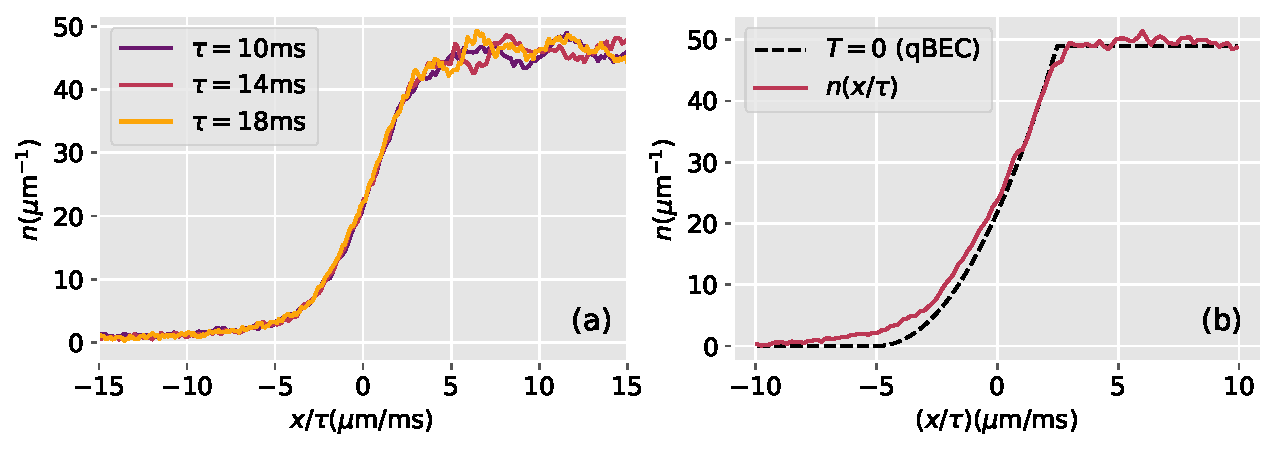
\includegraphics[width=1.0\linewidth]{figures/06_Bipart/DWD_GPE_vs_exp_V2.pdf}
\caption{
(a) Profils de densité mesurés pour différents temps $t$, représentés en fonction de la variable $x/t$. L’excellent recouvrement des courbes confirme l’auto-similarité et la dynamique balistique.\\
(b) Comparaison entre un profil mesuré à $t = 10$~ms (points) et la prédiction GHD à température nulle (ligne), pour un paramètre de Lieb $\gamma = 4{,}6 \times 10^{-3}$.
}
\label{fig:euler}
\end{figure}

\paragraph{Conclusion}

Ces observations expérimentales confirment que la dynamique induite par une coupure bipartite est bien décrite par la GHD à l’échelle d’Euler, dans un régime temporel intermédiaire bien identifié. La mise à l’échelle en $x/t$ permet une confrontation directe entre théorie et expérience, et ouvre la voie à des tests plus précis des effets thermiques et des corrections hors-échelle d’Euler.

\subsection*{Résumé}

Nous avons étudié la dynamique hors équilibre d’un gaz unidimensionnel de bosons à la suite d’une coupure bipartite, créant une discontinuité initiale dans le profil de densité. Cette configuration, analogue au problème de Riemann quantique, engendre une évolution balistique décrite par la Théorie Hydrodynamique Généralisée (GHD).

Sur le plan expérimental, nous avons mis en œuvre un protocole précis pour préparer un gaz homogène, le scinder spatialement à l’aide d’un DMD, puis le libérer dans un guide unidimensionnel. L’évolution du profil de densité $n(x,t)$ a été mesurée pour différents temps, révélant une structure auto-similaire caractéristique du régime hydrodynamique.

Côté théorique, nous avons présenté les équations de GHD dans leur forme convective, et montré que la solution du problème de Riemann s’exprime sous la forme d’une distribution auto-similaire $\nu(x/t, \theta)$. Cette structure permet de prédire analytiquement les profils de densité.

La comparaison entre les données expérimentales et les prédictions de la GHD à température nulle montre une excellente correspondance dans un régime temporel intermédiaire bien défini ($t \in [6,18]$~ms). Ces résultats valident la GHD comme cadre pertinent pour décrire la relaxation balistique de systèmes quantiques intégrables, et ouvrent la voie à des explorations plus fines des effets thermiques et quantiques hors équilibre.



\section{Sonder la distribution locale des rapidités}
\label{sec:local}

{\color{blue}
Points clés :
\begin{itemize}
	\item Protocole expérimental pour extraire une tranche locale du gaz après évolution.
	\item Expansion 1D de la tranche sélectionnée et reconstruction de la distribution de rapidités $\Pi(\theta)$.
	\item Comparaison avec les prédictions GHD : asymétrie, effet de la largeur finie de la tranche, et limitations dues à la résolution et aux effets diffusifs.
	\item Discussion sur les écarts observés et les hypothèses du modèle.
\end{itemize}

}


\subsection*{Introduction}
\ref{chap6:sec:ghd}
Les outils de l'hydrodynamique généralisée (GHD) introduits dans la section~\ref{chap6:sec:ghd} permettent de décrire la dynamique hors équilibre dans des configurations de type jonction bipartite.
Dans le scénario de jonction bipartite — où deux parties du gaz, initialement préparées dans des états thermodynamiques distincts, sont soudainement mises en contact — la dynamique engendre des profils locaux fortement hors équilibre. En particulier, lorsque l’état initial consiste en un gaz homogène à droite et une région vide à gauche, la GHD prédit qu’à grand temps le système atteint un régime stationnaire autosimilaire, dans lequel les observables locales dépendent uniquement du rapport $\zeta = x/t$. Dans ce régime, la distribution locale des quasi-particules est décrite par un facteur d’occupation $\nu^*(\zeta,\theta)$, solution d’une équation de type~\eqref{eq:nuetoile}.

\medskip

Une prédiction remarquable de ce cadre est la présence, du côté droit du système, d’une discontinuité abrupte dans la distribution en rapidité du facteur d’occupation~$\nu^*(\zeta,\theta)$ — signature d’un état local proche du fondamental. À l’inverse, du côté gauche (où le gaz est initialement absent), la distribution reste lisse en rapidité, ce qui indique un état localement excité, distinct d’un état fondamental. Ce contraste fort entre les deux régions — l’une présentant une distribution lisse, l’autre une discontinuité abrupte — reflète la propagation balistique des quasi-particules, conséquence directe de l’intégrabilité du système. En effet, dans un système intégrable, les quasi-particules conservent leur individualité et se propagent à vitesse bien définie sans diffusion, ce qui permet de maintenir à grand temps des structures non thermalisées comme des discontinuités, absentes dans les systèmes non intégrables.

\medskip

L’objectif de cette section est de confronter ces prédictions théoriques à l’expérience, en accédant à la distribution locale de rapidités du gaz. Pour cela, nous mettons en œuvre un protocole expérimental inspiré de la Réf.~\cite{dubois_probing_2024}, permettant de mesurer indirectement cette distribution via l’expansion libre d’une tranche localisée du gaz. En parallèle, nous réalisons des simulations numériques de la dynamique à l’aide de la GHD, ce qui nous permet de comparer les distributions mesurées avec les prédictions théoriques, et ainsi de tester la présence effective de la discontinuité attendue.

\medskip

{\color{blue}
Nous structurons cette analyse en quatre étapes principales :
\begin{itemize}
    \item Sélection d’une tranche localisée du gaz après un temps d’évolution donné.
    \item Observation du profil de vitesse après expansion libre, révélant une éventuelle asymétrie.
\end{itemize}
}

\begin{figure}[!htb]
\centering
\begin{tikzpicture}
    \node[rectangle, draw = none] (bord) at (0,0) {
        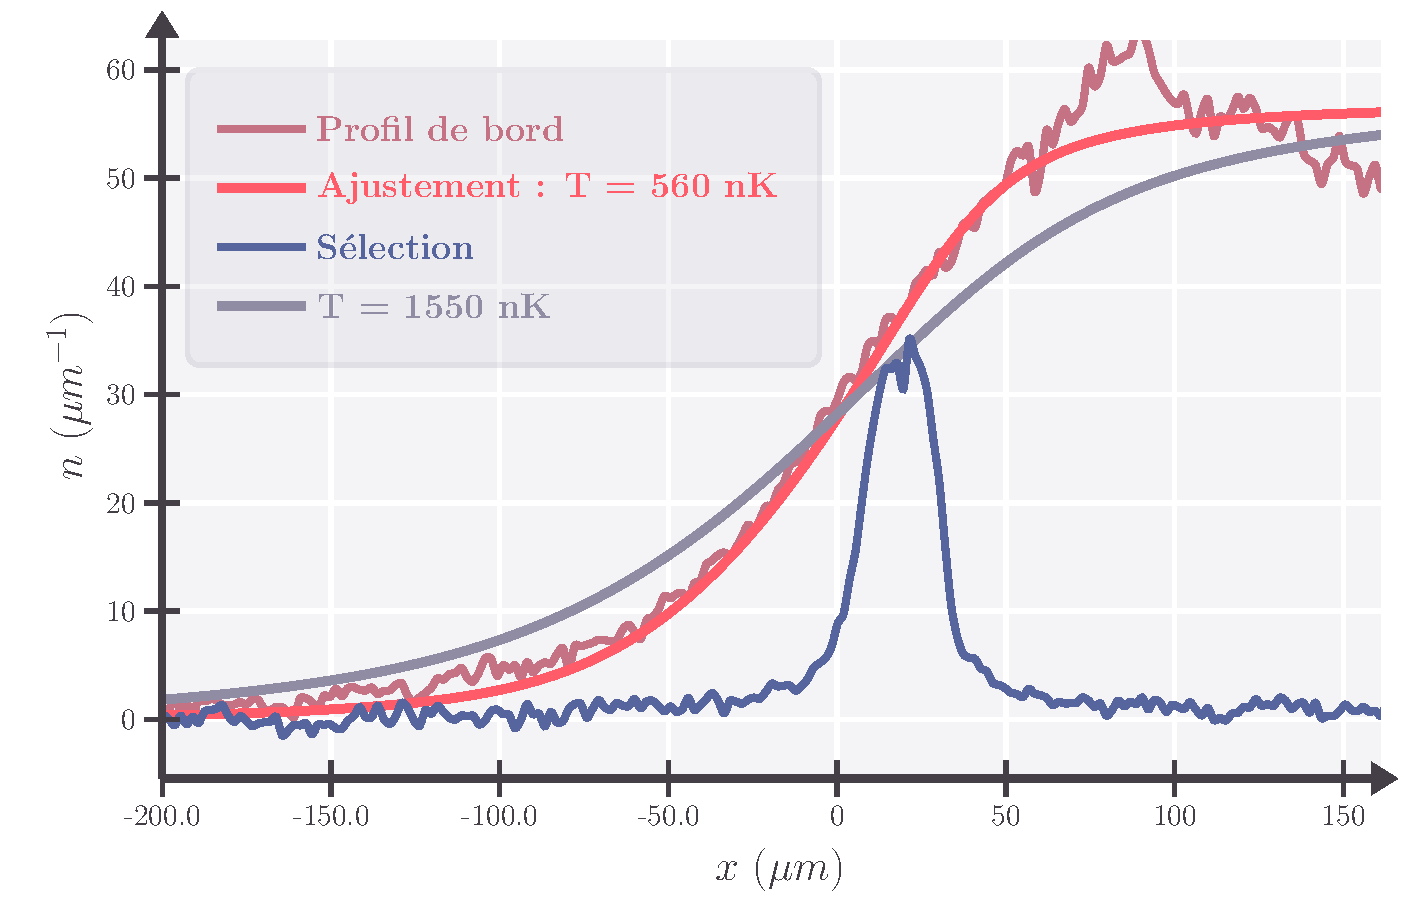
\includegraphics[width=0.5\textwidth , page = 1]{figures/06_Bipart/Figures}
    };
    \node[circle, draw=none, above=0cm of bord , shift={( -2.5cm , -0.5cm )} ] {(a)};
    
    \node[right=1mm of bord , shift={( -0.5cm , 0cm )}] (assy) {
        \includegraphics[width=0.5\textwidth , page = 2 ]{figures/06_Bipart/Figures}
    };
    \node[circle, draw=none, above=0cm of assy , shift={( -2.5cm , -0.5cm )}] {(b)};
\end{tikzpicture}
\caption{(a) {\it Profil de bord et tranche sélectionnée.} Le profil de bord après $18\,\mathrm{ms}$ est montré en rouge. L'ajustement thermique donne une température $T = 560\,\mathrm{nK}$ (orange). Le profil de densité mesuré $1\,\mathrm{ms}$ après la sélection de la tranche est en bleu. (b) {\it Asymétrie du profil d’expansion de la tranche.} Le profil de densité après une expansion pendant $\tau = 30\,\mathrm{ms}$ est comparé à son image miroir. Le centre de symétrie $x_s = -17\,\mu$m minimise la distance quadratique $\delta^2 = \int dx\, (\tilde{n}(x) - \tilde{n}(2x_s - x))^2$.}
\label{fig:simul_deformation}
\end{figure}



%\subsection{Protocol experimental}

\subsection{Sélection d’une tranche localisée après déformation du bord}

{\color{blue}
Nous laissons d’abord le gaz se dilater pendant un temps $t=18~\mathrm{ms}$, de sorte que le bord s’étale sur une large zone d’environ $350~\mathrm{\mu m}$, comme illustré en Fig.~\ref{fig:BiPart.coupure1} (e)-(f) et  Fig ~\ref{fig:simul_deformation} (a).  
Nous sélectionnons ensuite une tranche du gaz comprise dans l’intervalle $[x_0-\ell/2, x_0+\ell/2]$, en éliminant tous les atomes situés hors de cette tranche à l’aide d’un faisceau de poussée~\cite{dubois_probing_2024}(Fig \ref{fig:BiPart.coupure2} (a)--(c)). 
 

}


\paragraph{Sélection locale d'une tranche du gaz.}

Afin d’accéder localement à la distribution de rapidité, nous exploitons le fait qu’après un temps $t = 18~\mathrm{ms}$, le bord du gaz s’étale sur plusieurs centaines de microns — environ $350~\mathrm{\mu m}$ — comme illustré en Fig.~\ref{fig:BiPart.coupure1}(e)-(f) et Fig.~\ref{fig:simul_deformation}(a). Cette large extension spatiale permet d’identifier des régions à la fois assez étendues pour être sélectionnées expérimentalement, et suffisamment étroites pour que le gaz puisse y être considéré comme localement homogène dans le cadre de l’hydrodynamique généralisée.

\medskip
\noindent
Pour isoler une telle région, un {\bf faisceau de poussée} est appliqué afin d’{\bf éliminer tous les atomes situés hors d’un intervalle spatial} centré en $x_0 = 18~\mu\mathrm{m}$ et de largeur $\ell$. Cette technique, inspirée de la Réf.~\cite{dubois_probing_2024}, permet de ne conserver qu’une {\bf tranche localisée du gaz}, dont la distribution en rapidité reflète l’état local $\rho(x,\theta)$ aux abords de $x \approx x_0$, comme illustré en Fig.~\ref{fig:BiPart.coupure2}(a)--(c).


\medskip
\paragraph{Contrôle expérimental du faisceau de sélection.}

La sélection spatiale du gaz est réalisée à l’aide d’un dispositif à micro-miroirs (DMD), qui permet de contrôler finement la forme du faisceau de poussée utilisé pour éliminer les atomes hors d’un intervalle centré en $x_0$. Ce dispositif est piloté via une interface logicielle développée au sein de l’équipe, basée sur les outils \textsc{Cicero-Iso} et \textsc{Spartacus}. Le DMD est commandé par une série de paramètres expérimentaux transmis à ces logiciels, dont certains (comme la position $x_0$) sont enregistrés systématiquement au cours de l’expérience. En revanche, d'autres paramètres, notamment la largeur effective $\ell$ du faisceau, n’ont pas été archivés dans la base de données associée aux séquences expérimentales. Ainsi, dans les paragraphes précédents, nous avons pu indiquer précisément la valeur de $x_0$ (ici $x_0 = 18~\mu\mathrm{m}$), mais non celle de $\ell$. Cette valeur sera déterminée a posteriori par analyse des profils expérimentaux, et jouera un rôle essentiel dans les simulations numériques présentées plus loin.

\medskip
\paragraph{Inhomogénéité de la tranche sélectionnée}

Dans l'idéal, on souhaiterait que l’intervalle de sélection soit suffisamment fin pour garantir l’homogénéité de la densité locale au sein de la tranche. Toutefois, comme la valeur exacte de $\ell$ n’a pas été enregistrée, nous ne pouvons pas l’estimer directement à partir des données de Fig.~\ref{fig:simul_deformation}(a), qui représente l’état du système avant sélection. Néanmoins, cette même figure montre également le profil de densité mesuré une milliseconde après la sélection. Or, comme nous le verrons dans la suite, les simulations GHD montrent que, dans cet intervalle de temps, la distribution en espace réel ne subit ni déplacement significatif, ni déformation notable. Il est donc raisonnable d’utiliser ce profil post-sélection comme estimation fidèle de la densité initiale dans la tranche.

\medskip
\paragraph{Estimation de la largeur $\ell$ et conséquences}

À partir de cette analyse, nous pouvons estimer que la largeur $\ell$ de la tranche sélectionnée est de l’ordre de $20$ à $30~\mu\mathrm{m}$. Or, pour une position centrale $x_0 \approx 18~\mu\mathrm{m}$, la densité atomique $\tilde{n}(x ; \tau = 0 )$ varie sensiblement sur cette échelle. La tranche sélectionnée n’est donc pas localement homogène, et la distribution de rapidité mesurée correspond en réalité à une moyenne spatiale de $\rho(x,\theta)$ sur un intervalle de largeur $\ell$ centré en $x_0$. Cette observation est essentielle pour l’interprétation des données et sera prise en compte dans la suite, en particulier dans les comparaisons avec les simulations hydrodynamiques.


\subsection{Expansion de la tranche et observation d’une asymétrie}

\paragraph{Principe de l’expansion et lien avec la distribution en rapidité}

Après la sélection, la tranche est laissée en expansion libre unidimensionnelle pendant un temps $\tau$, puis son profil de densité longitudinal $\tilde{n}(x,\tau)$ est mesuré. Cette expansion permet de convertir l’information spatiale en une information sur la distribution en rapidité. En effet, pour un temps $\tau$ suffisamment grand, on s’attend à ce que la densité observée soit proportionnelle à la distribution totale des rapidités dans la tranche :
\begin{equation}
\tau\, \tilde{n}(\tau \theta - x_0 ; \tau) \underset{\tau \to \infty}{\longrightarrow} \Pi(\theta),
\end{equation}
où, quel que soit le temps d'expansion unidimensionnelle $\tau$, la distribution de rapidité extensive $\Pi(\theta)$ reste constante, c’est-à-dire  $\Pi(\theta) = \int \rho(x, \theta ; \tau \geq 0)\, dx $. En particulier, cette distribution s’identifie à celle de l’état initial dans la tranche sélectionnée :
\begin{equation}
\Pi(\theta)  = \int_{x_0 - \ell/2}^{x_0 + \ell/2} \rho(x, \theta ; \tau = 0)\, dx.
\end{equation}
Autrement dit, $\Pi(\theta)$ correspond à la distribution de rapidité intégrée sur la tranche sélectionnée, conservée lors de l’expansion.

\paragraph{Observation expérimentale de l’asymétrie}

La théorie prédit que la distribution locale de quasi-particules $\rho(x,\theta)$ est fortement asymétrique en $\theta$. Cette asymétrie se retrouve dans $\Pi(\theta)$ et doit donc se manifester dans le profil d’expansion $\tilde{n}(x,\tau)$. Cette asymétrie est effectivement observée dans nos données expérimentales, comme illustré en Fig.~\ref{fig:simul_deformation}(b) pour un temps d’expansion $\tau = 30~\mathrm{ms}$. 


\subparagraph{Quantification de l’asymétrie par symétrisation.}
La figure \ref{fig:simul_deformation}(b) présente deux courbes : le profil mesuré $\tilde{n}(x)$ (abréviation de $\tilde{n}(x,\tau)$) et son image par symétrie par rapport à un axe $x = 2x_s$. L’objectif est de rendre visible et de quantifier l’asymétrie du profil.
Pour ce faire, nous considérons une décomposition naturelle du profil autour d’un centre $x = x_s$ :
\begin{equation}
\tilde{n}(x) = \tilde{n}_{\text{pair}}^{(x_s)}(x) + \tilde{n}_{\text{impair}}^{(x_s)}(x),\quad \mbox{où} \, \left\{\begin{array}{lcr}\tilde{n}_{\text{pair}}^{(x_s)}(x) &=&  \displaystyle \frac{\tilde{n}(x) + \tilde{n}(2x_s - x)}{2} , \\ \tilde{n}_{\text{impair}}^{(x_s)}(x) &=& \displaystyle \frac{\tilde{n}(x) - \tilde{n}(2x_s - x) }{2}\end{array} \right. .
\end{equation}

Cette décomposition correspond à une projection du profil sur les fonctions paires et impaires centrées en $x = x_s$.

L’asymétrie du profil est directement liée à la composante impaire. Pour la quantifier, nous cherchons la valeur de $x_s$ qui minimise la norme $L^2$ de la partie impaire :
\begin{equation}
\mathcal{\delta}^2(x_s) = \int dx\, \left[\tilde{n}(x) - \tilde{n}(2x_s - x)\right]^2.
\end{equation}
La valeur optimale de $x_s$ minimise cette fonctionnelle $\mathcal{\delta}^2(x_s)$ et fournit un axe de symétrie effectif pour le profil. Cette méthode permet de comparer de manière robuste différentes conditions expérimentales, ou différents temps d’expansion, en s’affranchissant d’un ajustement arbitraire de centre.


\subparagraph{Effet de l’homogénéité de la tranche sélectionnée}

Plus la densité atomique est homogène dans la tranche sélectionnée, plus l’expansion est asymétrique et restitue fidèlement la distribution de rapidité au point $x_0$. En effet, si $\rho(x,\theta)$ est uniforme sur la largeur $\ell$, on obtient :
\begin{equation}
\Pi(\theta) \simeq \ell\, \rho(x_0,\theta) \quad \Rightarrow \quad \tau\, \tilde{n}(\tau \theta - x_0 ; \tau) \simeq \ell\, \rho(x_0,\theta),
\end{equation}
ce qui permet d’accéder directement à la distribution locale, y compris à d’éventuelles discontinuités.

Deux stratégies permettent d’améliorer cette homogénéité :
\begin{itemize}[label = $\bullet$] 
    \item Diminuer la largeur $\ell$ de la sélection,
    \item Augmenter le temps $t$ de déformation du bord avant sélection, pour étendre la région d’intérêt spatialement.
\end{itemize}
Cependant, ces deux approches ont des limitations : une plus petite valeur de $\ell$ réduit le nombre d’atomes sélectionnés, ce qui diminue le rapport signal/bruit, et des temps $t$ trop longs font sortir le système du régime semi-infini, introduisant des effets de bord non désirés (voir Fig.~[à insérer]).

\subparagraph{Limites sur le temps d’expansion}

Allonger le temps d’expansion $\tau$ permet d’approcher plus fidèlement le régime asymptotique $\tau \to \infty$ où la correspondance avec $\Pi(\theta)$ est exacte. Toutefois, cette expansion est limitée expérimentalement par la taille longitudinale du confinement 1D, de l’ordre de $1~\mathrm{mm}$, correspondant à la taille typique des triplets de microfils. Comme illustré en Fig.~\ref{fig:simul_deformation}(b), le nuage atteint cette taille à $\tau \sim 30~\mathrm{ms}$, ce qui constitue une limite pratique. Par ailleurs, des simulations GHD (voir Ref.~\cite{dubois_probing_2024}) montrent que des temps significativement plus longs seraient nécessaires pour que $\tau \tilde{n}$ converge véritablement vers $\Pi(\theta)$.

\subparagraph{Renforcer l’asymétrie observée}

Enfin, une asymétrie plus marquée peut être obtenue en modifiant l’état initial du gaz. En particulier, une bipartition réalisée à partir d’un état initial plus excité (c’est-à-dire moins proche du fondamental) du côté gauche renforcerait le contraste entre les deux côtés. Cette stratégie permettrait d’amplifier la discontinuité attendue dans la distribution de rapidité, et donc dans le profil d’expansion.

\vspace{1em}
\begin{center}
\textit{[Figure : asymétries observées pour différents états initiaux]}
\end{center}

\subsection*{Résumé}

Dans cette section, nous avons présenté un protocole permettant de sonder la distribution locale des quasi-particules dans un gaz unidimensionnel hors équilibre, en sélectionnant une tranche étroite après déformation du bord, puis en la laissant s’étendre librement. Cette procédure permet d’accéder indirectement à la distribution intégrée en rapidité $\Pi(\theta)$ dans la tranche, et de tester les prédictions de la GHD sur la structure locale du facteur d’occupation $\nu(x,\theta)$.

L’analyse expérimentale révèle une forte asymétrie du profil d’expansion, signature d’une distribution de rapidité non thermique. La méthode de symétrisation introduite permet de quantifier cette asymétrie de manière robuste. Nous avons montré que l’homogénéité de la tranche sélectionnée, la durée d’expansion libre, ainsi que l’état initial du gaz influencent fortement l’observation de cette asymétrie.

Enfin, ces résultats confirment qualitativement les prédictions de la GHD dans le régime stationnaire autosimilaire, en particulier l’existence d’une discontinuité du côté du gaz initialement présent, tout en mettant en évidence les limitations expérimentales et les effets hors modèle — notamment les contraintes liées à la sélection spatiale et à la durée d’expansion.

\medskip

Pour approfondir cette analyse, nous nous appuyons à présent sur des simulations numériques basées sur l’équation de GHD. Celles-ci permettent de modéliser la dynamique complète de la tranche sélectionnée, depuis la déformation du bord jusqu’à son expansion, et de confronter quantitativement les distributions mesurées aux prédictions théoriques.


\section{Simulations numériques}
\label{sec:simulations}

Cette section présente en détail les étapes nécessaires à la résolution numérique de l’équation de GHD dans le cadre des simulations effectuées.

Dans un premier temps, nous explicitons le calcul du facteur d’occupation $\nu(\theta)$ et de la densité de rapidité $\rho(\theta)$ à l’équilibre thermique, obtenus à partir d’un couple $(T, \mu)$ donné.

Nous décrivons ensuite l’évolution du système sous l’effet du potentiel de piégeage : en particulier, nous nous intéressons à la dynamique du contour délimitant la région occupée dans l’espace des phases $(x, \theta)$, en exploitant la conservation lagrangienne du facteur d’occupation.

La simulation permet alors de suivre la déformation du bord au cours du temps. Une fois ce bord suffisamment évolué, nous extrayons une tranche du système pour en simuler l’expansion.

Enfin, nous comparons la distribution de rapidité issue de cette expansion numérique avec celle mesurée expérimentalement, dans des conditions analogues.


\subsection{Système homogène à l'équilibre thermique}

Nous considérons d’abord un gaz unidimensionnel homogène infini, à l’équilibre thermique, caractérisé par un couple de paramètres thermodynamiques $(T, \mu)$. La thermodynamique de Bethe-Ansatz permet de décrire un tel système par une équation intégrale sur le poids/potentiel spectral $w(\theta)$, donnée par :
\begin{equation}
w(\theta) = \beta\left(\frac{1}{2}m\theta^2 - \mu\right),
\end{equation}
où $\beta = (k_B T)^{-1}$ est l’inverse de la température (en unités d’énergie). La résolution de cette équation donne accès au facteur d’occupation $\nu_0(\theta)$ .

À partir de $\nu_0(\theta)$, les densités de quasi-particules $\rho(\theta)$ et de niveaux disponibles $\rho_s(\theta)$ sont obtenues par un processus de {\bf habillage} (ou {\bf dressing}) standard (voir section~\ref{para-algho-TBA}). Ces grandeurs sont ensuite utilisées pour calculer les observables physiques.



\paragraph{Détermination du potentiel chimique à température fixée}

Dans l’expérience, la quantité accessible est la densité linéique homogène $n_0$, par exemple $n_0 = 56~\mu\mathrm{m}^{-1}$ (voir Fig.~\ref{fig:simul_deformation}(a)). Afin de reproduire cette densité dans les simulations, nous fixons la température $T$ (déterminée indépendamment dans l’expérience), puis nous ajustons la valeur du potentiel chimique $\mu$ pour satisfaire la contrainte :
\begin{equation}
n_0 = \int \rho_0(\theta)\, d\theta.
\end{equation}

Ce processus est effectué numériquement en résolvant les équations TBA pour différentes valeurs de $\mu$ jusqu’à obtenir l’accord avec la densité cible. Dans notre cas, pour $T = 560~\mathrm{nK}$, nous obtenons $\mu = 65~\mathrm{nK}$ comme valeur correspondant à la densité $n_0 = 56~\mu\mathrm{m}^{-1}$.

Les résultats de cette résolution sont illustrés en Fig.~\ref{fig:BiPart.insitut} :
\begin{itemize}[label = $\bullet$]
    \item Le facteur d’occupation obtenu $\nu_0(\theta)$ est représenté en (a).
    \item La densité spatiale correspondante, constante dans le cas homogène, est illustrée en (b).
    \item Le facteur $\nu_0(\theta)$ est à nouveau tracé en (c), en complément pour lecture directe.
\end{itemize}

Dans ce régime homogène, la distribution est indépendante de la position, i.e.
\begin{equation}
\nu(x, \theta) = \nu_0(\theta), \quad \forall x,
\end{equation}
comme visible en Fig.~\ref{fig:BiPart.insitut}(a,c).


\begin{figure}[!htb]
	\centering
	\includegraphics[width=0.5\textwidth , page = 4 ]{figures/06_Bipart/Shema.pdf}	
	\caption{a) Facteur d’occupation initial $\nu(x, \theta) = \nu_0(\theta)$ correspondant à un état d’équilibre thermique à la température $T = 560~\mathrm{nK}$, pour une densité linéique homogène $n_0 = 56~\mu\mathrm{m}^{-1}$. Ces paramètres correspondent à une potentielle chimique $\mu = 65~\mathrm{nK}$.
b) Densité spatiale linéique $n(x) = \int \rho_{[\nu]}(x, \theta)\, d\theta$, constante et égale à $n_0 = 56~\mu\mathrm{m}^{-1}$.
c) Facteur d’occupation $\nu_0(\theta)$ correspondant à la distribution thermique illustrée en a).}
	\label{fig:BiPart.insitut}
\end{figure}


\subsection{Dynamique du contour dans l’espace des phases $(x, \theta)$.}
\label{sec:contour_GHD}

Une fois le facteur d’occupation initial $\nu_0(\theta)$ déterminé, nous cherchons à décrire l’évolution temporelle de la région occupée dans l’espace des phases $(x,\theta)$. Cette région, notée $\Gamma_t$, est définie comme le support du facteur d’occupation $\nu(x,\theta,t)$ : elle contient l’ensemble des points pour lesquels $\nu$ est non nul à l’instant $t$.

\paragraph{Interprétation lagrangienne et trajectoires caractéristiques :.}
Dans l’hydrodynamique généralisée, l’évolution de $\nu$ est décrite par une équation de transport pur du type \eqref{eq:nu.cont}. Cette équation peut être interprétée selon une perspective \textbf{lagrangienne} :  le facteur d’occupation $\nu$ reste constant au cours du temps c'est à dire  
\begin{eqnarray}\label{chap6:eq:traj_lagr_0}
	 \nu ( x(t) , \theta(t) ; t ) = \nu ( x(0) , \theta(0) ; 0 ) 
\end{eqnarray}
lorsqu’on suit les trajectoires $(x(t), \theta(t))$ définies par :  
\begin{eqnarray*}
	\frac{d \nu}{dt} (x , \theta ; t ) = 0,	
\end{eqnarray*}

soit $\partial_t \nu + \dot{x} \partial_t \nu = 0$ soit en identifiant dans \eqref{eq:nu.cont}:
\begin{equation}
\label{chap6:eq:traj_lagr_1}
\partial_t \left( \begin{array}{c} x(t) \\ \theta(t) \end{array} \right)  =  \left( \begin{array}{c} v^{\mathrm{eff}}_{[\nu]}(\theta(t)) \\ 0 \end{array} \right)\, \mbox{soit} \quad \left\{ \begin{array}{rcl}
\displaystyle \frac{d x}{dt}(t) & = & v^{\mathrm{eff}}_{[\nu]}(\theta), \\
\theta(t) & = & \theta(0) \equiv \theta.
\end{array} \right. 
\end{equation}
%où $s$ est un paramètre pour différentier les particules fluide dans la perspective lagrangienne. Cette dernière équation \eqref{chap6:eq:traj_lagr_1} implique que 
%\begin{equation}
%\label{chap6:eq:traj_lagr_2} 
%\left\{ \begin{array}{rcl}
%\displaystyle \frac{d x}{dt}(s;t) & = & v^{\mathrm{eff}}_{[\nu]}(\theta(s)), \\
%\theta(s;t) & = & \theta(s;0) = \text{constante}.
%\end{array} \right.
%\end{equation}

Autrement dit, les quasi-particules de rapidité $\theta$ se déplacent à la vitesse efficace $v^{\mathrm{eff}}_{[\nu]}$, et leur répartition reste inchangée tout au long de leur trajectoire dans l’espace des phases. Cette conservation est analogue à une conservation lagrangienne classique, où l’on suit un élément de fluide individuellement.

\medskip

\paragraph{État initial en "patch" et Propagation du support .}
Nous considérons un état initial de type « patch » : le facteur d’occupation $\nu(x ,\theta ;0)$ est égal à $\nu_0(\theta)$ à l’intérieur d’une certaine région initiale $\Gamma_0$, et nul en dehors. Ce choix modélise une situation typique de type « front d’onde » avec un gaz localement homogène dans une portion de l’espace.

En suivant chaque point $(x(t),\theta)$ de cette région selon l’équation~\eqref{chap6:eq:traj_lagr_1}, on détermine la région atteinte à l’instant $t$, notée $\Gamma_t$. Par construction, le facteur d’occupation reste constant le long de ces trajectoires d'après \eqref{chap6:eq:traj_lagr_0}, $\nu(x(t),\theta,t) = \nu(x(0),\theta,0)$  soit :

\begin{equation}
	\nu(x(t),\theta,t)  = \nu_0(\theta).
\end{equation}

Par conséquent, on peut écrire l’évolution du facteur d’occupation de manière explicite :

\begin{equation}
\label{eq:contour_support}
\nu(x, \theta, t) =
\begin{cases}
\nu_0(\theta) & \text{si } (x,\theta) \in \Gamma_t, \\
0 & \text{sinon}.
\end{cases}
\end{equation}

Cette propriété est une conséquence directe du cadre intégrable sous-jacent et de la forme particulière de l’équation de GHD, qui assure que les caractéristiques $(x(t),\theta)$ suivent une dynamique conservant localement l’occupation.

\medskip

Enfin, notons que, dans ce cadre, la vitesse efficace $v^{\mathrm{eff}}_{[\nu]}(x,\theta,t)$ est fonctionnelle du facteur d’occupation \textit{instantané}. Toutefois, dans les cas où $\nu$ conserve sa structure initiale par blocs (comme ici avec un contour net), on peut exprimer cette vitesse uniquement à partir de $\nu_0$ sur chaque trajectoire, ce qui permet de déterminer toute la dynamique sans recalculer le champ $\nu$ à chaque pas de temps. Cette remarque est à la base des méthodes numériques efficaces employées dans nos simulations (voir section~\ref{sec:simu_bord}).


\subsection{Simulation de la déformation du bord}

Dans la configuration initiale correspondant à l'expérience de déformation du bord (Fig.~\ref{fig:BiPart.coupure1}), la région occupée par le gaz correspond à \(x > 0\), avec un facteur d’occupation uniforme \(\nu(x,\theta; t=0) = \nu_0(\theta)\) pour \(x > 0\), et nul pour \(x < 0\). Le contour initial séparant ces deux domaines est donné par \((x = 0, \theta)\). L’évolution de ce front peut être entièrement décrite à l’aide de l’équation de GHD, en supposant que le contour reste bijectif au cours du temps.


Nous paramétrons ce contour par une variable \(s\), de sorte que le bord à l’instant \(t\) est donné par \((x_b(s;t), \theta_b(s))\), avec \(\theta_b(s)\) strictement croissante (i.e. \((x_b(s;t), \theta_b(s)) \in \partial \Gamma_t\)).  
La conservation lagrangienne du facteur d’occupation implique que la vitesse efficace \(v^{\mathrm{eff}}_{[\nu^\ast]}(\theta_b(s))\) est indépendante du temps de déformation \(t\).  
En dérivant \eqref{eq:traj_lagr}, on obtient que chaque point \((x_b(s;t), \theta_b(s))\) suit une trajectoire caractéristique associée à cette vitesse efficace :
\[
x_b(s;t) = v^{\mathrm{eff}}_{[\nu^\ast]}(\theta_b(s)) \cdot t,
\]
où \(\nu^\ast(v, \theta)\) désigne le facteur d’occupation exprimé dans les variables autosimilaires, avec \(v = x/t\).
Le facteur d’occupation autosimilaire prend alors la forme \eqref{eq:contour_support} :
\begin{equation}
\label{eq:contour_bord_sim}
\nu^\ast(x_b(s;t)/t,\theta)  =  	 \begin{cases} \nu_0(\theta) & \text{si }  \theta < \theta_b(s) \\ 0 & \text{sinon} \end{cases}, \, \quad \mbox{soit} \quad  	
\nu^\ast(v,\theta) = 
\begin{cases}
\nu_0(\theta) & \text{si }  v < v^{\mathrm{eff}}_{[\nu^\ast]}(\theta), \\
0 & \text{sinon} .
\end{cases}
\end{equation}
La vitesse efficace \(v^{\mathrm{eff}}_{[\nu^\ast]}(\theta)\) est déterminée par :
\(
v^{\mathrm{eff}}_{[\nu^\ast]}(\theta) = \frac{\mathrm{id}^{\mathrm{dr}}_{[\nu^\ast]}(\theta)}{\mathrm{1}^{\mathrm{dr}}_{[\nu^\ast]}(\theta)}.
\)
À partir de la connaissance du contour \((x_b(s;t), \theta_b(s))\), on reconstruit le facteur d’occupation \(\nu(x,\theta; t)\) à l’aide de l’équation~\eqref{eq:contour_bord_sim} (Fig. \ref{fig:BiPart.coupure1}~(e) $\&$(g)). On en déduit ensuite la densité totale de quasi-particules par :
\(
\rho_s(x,\theta;t) = \frac{\hbar}{m} \cdot 1^{\mathrm{dr}}_{[\nu]}(\theta),
\,
\rho(x,\theta;t) = \nu(x,\theta;t) \cdot \rho_s(x,\theta;t),
\)
puis la densité linéique :
\(
n(x,t) = \int \rho(x,\theta;t)\, d\theta.
\)
(Fig. \ref{fig:BiPart.coupure1}~(e)$\&$(f)).

\medskip 

Enfin, en fixant \(n_0 = 56~\mu\mathrm{m}^{-1}\), nous ajustons la température \(T\) des simulations GHD pour reproduire les données expérimentales de déformation du bord (Fig.~\ref{fig:simul_deformation}). Cet ajustement donne \(T = 560~\mathrm{nK}\).

\begin{figure}[!htb]
	\centering
	\includegraphics[width=\textwidth , page = 5 ]{figures/06_Bipart/Shema.pdf}
	\caption{
(a) À l'instant $t = 0^+$, immédiatement après le « quench bipartite » en $x = 0$, le facteur d'occupation est donné par $\nu(x, \theta ; t = 0^+) = \nu_0(\theta)$ pour $x > 0$ et est nul pour $x < 0$. Le bord initial représenté en tirets par l'ensemble des points $(x_b(s; t = 0^+) = 0,\ \theta(s; t = 0^+))$.
(b) Densité spatiale linéique $n(x)$ : en pointillés, $n(x; t = 0^-) = \int \rho(x, \theta; t = 0^-) \, \mathrm{d}\theta = n_0 = 56~\mu\mathrm{m}^{-1}$ juste avant le quench ; en ligne pleine, $n(x; t = 0^+) = n_0$ pour $x > 0$ et $0$ pour $x < 0$.
(c) À gauche de la coupure ($x < 0$) : en pointillés, $\nu(x, \theta ; t = 0^-) = \nu_0(\theta)$ ; en ligne pleine, $\nu(x, \theta ; t = 0^+) = 0$.
(d) À droite de la coupure ($x > 0$), le facteur d'occupation reste inchangé : $\nu(x, \theta ; t = 0^+) = \nu_0(\theta)$.
(e) À l'instant $t = 18~\mathrm{ms}$, après l'évolution balistique post-quench, le facteur d'occupation est donné par $\nu^\ast(x_b(s;t)/t, \theta) = \nu_0(\theta)$ pour $\theta < \theta_b(s;t)$, et nul pour $\theta > \theta_b(s;t)$, résolvant l'équation~(\ref{eq:nuetoile}), pour $t>0$. $\nu(x(s;t), \theta(s;t))(=\nu^\ast(x(s;t)/t, \theta(s;t)))$ est invarient de la déformation ie de $t>0$.  Le bord représenté en tirets par l'ensemble des points $(x_b(s; t)/t,\, \theta(s; t))$. Étant donné que la coupure initiale est en $x = 0$ et que l’évolution du bord est balistique, cette courbe résoud $v^{\mbox{\tiny eff}}_{[\nu^\ast(x(s; t)/t, \cdot) ]}(\theta(s; t)) = x(s; t)/t = v(s)$ (\ref{eq:nu.cont}).
(f) Densité spatiale  $n^\ast(x/t)$ en régime hydrodynamique (scaling).
(g) Pour les atomes à droite de la coupure : en pointillés, $\nu^\ast(x(s;t)/t, \theta) = \nu_0(\theta)$ ; en ligne pleine, $\nu^\ast(x_b(s;t)/t, \theta) = \nu_0(\theta)$ pour $\theta < \theta_b(s;t)$ et nul pour $\theta > \theta_b(s;t)$. Le raisonnement est similaire pour les atomes à gauche de la coupure.
}
	\label{fig:BiPart.coupure1}
	
\end{figure}

\subsection{Simulation de l’expansion.}

Après la déformation du bord, une sélection spatiale est réalisée pour isoler une tranche du gaz (voir Fig.~\ref{fig:BiPart.coupure2}(a)), que l’on laisse ensuite se dilater librement en une dimension pendant un temps \(\tau\). Contrairement au cas de la déformation du bord, le contour de la région occupée dans $(x,\theta)$ n’est plus bijectif ($\partial \Gamma_t \ni (x,\theta) \mapsto \theta $ n'est pas injectif ): pour une position donnée de $x$, plusieurs rapidité $\theta$ peuvent exister telles que $(x,\theta)$ appartiennent au contour $\partial \Gamma_t$ de la région occupée.

Pour surmonter cette difficulté, nous décomposons le contour en deux branches bijectives : le bord gauche \((x_g(s;\tau), \theta_g(s))\) et le bord droit \((x_d(s;\tau), \theta_d(s))\). Cette décomposition garantit que sur chaque branche, la correspondance \(\theta \mapsto x\) est bijectif. Le facteur d’occupation après un temps \(\tau\) est alors donné par \eqref{eq:contour_support} :
\begin{equation}
\label{eq:contour_exp}
\nu ( x(s;\tau), \theta ) = 
\begin{cases}
\nu_0(\theta) & \text{si } \theta \in [\theta_g(s), \theta_d(s)], \\
0 & \text{sinon}.
\end{cases}
\end{equation}

La vitesse efficace dépend désormais explicitement du temps $\tau$ et de la position, puisqu’elle est fonction du facteur d’occupation local :
\[
v^{\mathrm{eff}}_{[\nu(x(s;\tau),\cdot)]}(\theta(s)),
\]
Pour résoudre numériquement \eqref{eq:traj_lagr} on est ici obligé d'induire des pas de temps $d\tau$ : 
\[
	x(\tau +d\tau ) = x(\tau ) + v^{\mathrm{eff}}_{[\nu(x(s;\tau),\cdot)]} (\theta(s))d \tau.
\]

En suivant l’évolution de chaque point du contour via cette vitesse, on reconstruit la densité spatiale \(n(x,\tau)\), à comparer aux données expérimentales (Fig.~\ref{fig:BiPart.coupure2}(f)).

\medskip

\paragraph{Détermination de la taille de la tranche \(\ell\).}

Les simulations d’expansion conservent le nombre de particules à mieux que \(3\%\). Comme mentionné précédemment, lors de l’expérience, nous avons enregistré la position du centre de la tranche \(x_0\), mais pas sa largeur \(\ell\).  
Nous avons donc choisi d’ajuster \(\ell\) de manière à ce qu’après expansion unidimensionnelle, le nombre total de particules prédit par les simulations coïncide avec celui mesuré expérimentalement dans la Fig.~\ref{fig:simul_expansion}(b).

\medskip

Une première simulation est réalisée avec la température \(T = 560~\mathrm{nK}\), obtenue précédemment par ajustement sur la déformation du bord.  
Pour reproduire correctement le nombre total de particules après une expansion unidimensionnelle de durée \(\tau = 30~\mathrm{ms}\), la largeur de la tranche doit être fixée à \(\ell = 24~\mu\mathrm{m}\). 

\medskip

Cette expansion unidimensionnelle est modélisée en supposant que le facteur d’occupation $\nu(x,\theta)$ est conservé localement au sein de la tranche sélectionnée. La figure~\ref{fig:BiPart.coupure2} illustre les différentes étapes de cette procédure.
Dans un premier temps, la tranche est extraite du bord du système, tel qu’il a évolué jusqu’à l’instant $t = 18~ms$ dans le piège. L’évolution unidimensionnelle à partir de cette condition initiale repose sur le transport lagrangien du bord dans l’espace des phases $(x,\theta)$, en l’absence de piégeage.

\begin{figure}[!htb]
	\centering
	\includegraphics[width=\textwidth , page = 6 ]{figures/06_Bipart/Shema.pdf}
	\caption{
(a) À l'instant $\tau = 0^+$, immédiatement après la sélection de la tranche centrée en $x = x_0$ et de largeur $\ell$, la distribution de rapidité localement résolue est donnée par $\rho(x,\theta ; \tau = 0^+) = \nu(x, \theta ; t = 18~\mathrm{ms}) \, \rho_s(x,\theta ; t = 18~\mathrm{ms})$ pour $\vert x - x_0 \vert < \ell/2$, et est nulle pour $\vert x - x_0 \vert > \ell/2$. Le bord gauche immédiatement après la sélection est représenté en pointillés par l’ensemble des points $(x_g(s; \tau = 0^+),\ \theta_g(s; \tau = 0^+))$, et le bord droit en tiret-point par l’ensemble des points $(x_d(s; \tau = 0^+),\ \theta_d(s; \tau = 0^+))$. Le bord complet est donc la concaténation de ces deux ensembles. 
(b) Densité linéique spatiale $\tilde{n}(x)$ : en pointillés, $n(x; t = 18~\mathrm{ms})$ juste avant la sélection ; en ligne pleine, $\tilde{n}(x; \tau = 0^+)$, égal à $n(x; t = 18~\mathrm{ms})$ pour $\vert x - x_0 \vert < \ell/2$ et nul ailleurs. 
(c) Distribution de rapidité après sélection, $\Pi(\theta) = \int \rho(x,\theta ; \tau)\,\mathrm{d}x$, invariante sous l’évolution unidimensionnelle, représentée en rouge. La distribution localement résolue en $x_b(s; \tau = 0^+)$, $\rho(x_b(s; \tau = 0^+), \theta ; \tau = 0^+)$, est représentée en pointillés. Cette distribution est localement conservée, i.e., $\rho(x(s; \tau), \theta(s; \tau))$ reste inchangée au cours de l’évolution unidimensionnelle, indépendamment de $\tau$. 
(e) Distribution localement résolue $\rho(x, \theta ; \tau = 30~\mathrm{ms})$ après une évolution unidimensionnelle de $30~\mathrm{ms}$. Le bord gauche est représenté en pointillés par les points $(x_g(s; \tau = 30~\mathrm{ms}),\ \theta(s; \tau = 30~\mathrm{ms}))$, et le bord droit en tiret-point par $(x_d(s; \tau = 30~\mathrm{ms}),\ \theta(s; \tau = 30~\mathrm{ms}))$. 
(f) Densité spatiale $\tilde{n}(x; \tau = 30~\mathrm{ms})$. 
(g) Distribution de rapidité $\Pi(\theta)$ après la sélection (identique à celle de (c)).
}
	\label{fig:BiPart.coupure2}
	
\end{figure}


\subsection{Comparaison aux données expérimentales et discussion}

Nous comparons dans cette section les profils de densité obtenus par simulation GHD à ceux mesurés expérimentalement après expansion d’une tranche extraite du bord du système.

\medskip

La Fig.\ref{fig:simul_expansion}(a) montre le profil d’expansion simulé à partir d’un état initial à température $T = 560~nK$, déterminée indépendamment par ajustement sur la déformation du bord (cf. Fig.\ref{fig:simul_deformation}). Le profil présente une forte asymétrie caractéristique, avec un bord droit abrupt et une densité qui s'annule au-delà d’une certaine position. Toutefois, cette chute est moins abrupte que celle de la distribution locale des rapidités $\rho(x, \theta)$ au centre de la tranche. Deux effets principaux expliquent cet élargissement :
\begin{itemize}
	\item[(i)] La distribution de rapidité n’est pas homogène dans la tranche, si bien que la distribution intégrée $\Pi(\theta) = \int \rho(x,\theta) \, dx $  diffère de $\ell \rho(x , \theta )$ , comme visible sur la Fig.~\ref{fig:simul_expansion}(a), ligne pleine versus pointillée ;
	\item[(ii)] Le temps d’expansion $\tau =30~ ms$ est fini, de sorte que la densité spatiale observée $\tilde{n}(x , \tau )$ diffère de la transformation directe $\Pi( (x-x_0)/\tau) /\tau $, comme le montre la comparaison entre les courbes rouge et marron dans la même figure.
\end{itemize}

\medskip

La Fig.~\ref{fig:simul_expansion}(b) compare la densité simulée à $T=560~nK$ avec les données expérimentales. Bien que la forme générale du profil soit qualitativement bien reproduite, des écarts significatifs apparaissent, en particulier autour de $x \simeq \pm 350 ~\mu m$, et jusqu’à 25$\%$ dans la région centrale.

\medskip

Afin d’améliorer cet accord, nous avons traité la température $T$ de l’état initial comme un paramètre libre, conjointement à la largeur de tranche $\ell$. L’ajustement donne une température apparente de $T=1550~nK$, représentée par la ligne magenta dans la Fig.~\ref{fig:simul_expansion}(b). Cette valeur permet de mieux reproduire le profil d’expansion, en particulier dans les régions périphériques.

Cependant, le profil au bord correspondant à cette température, présenté en Fig.~\ref{fig:simul_deformation}(a), est incompatible avec les observations expérimentales. En particulier, la courbure du bord simulé à cette température est beaucoup plus prononcée que celle mesurée. Ceci suggère que l’ajustement par température libre masque d'autres effets physiques non pris en compte dans le modèle.

\medskip

Une analyse plus fine du profil expérimental révèle la présence de queues asymétriques à droite, absentes des prédictions GHD à l’échelle d’Euler. Ces queues pourraient résulter de phénomènes hors du cadre du modèle, notamment :

\begin{itemize}
\item \textbf{Effets de sélection de tranche} : le faisceau de poussée utilisé pourrait chauffer localement les atomes en bordure, entraînant des distributions de rapidité plus étendues que prévu.
\item \textbf{Effets diffusifs} : dans les régions de forts gradients, notamment au bord du gaz, des termes de diffusion (omnis présents dans la GHD à l’échelle d’Euler) pourraient devenir significatifs. De telles corrections ont été proposées récemment pour modéliser la GHD au-delà de l’approximation eulérienne.
\end{itemize}

\medskip

En résumé, bien que la GHD reproduise globalement la forme du profil d’expansion, des écarts importants subsistent. Leur origine semble liée à des effets microscopiques non capturés par la description eulérienne — en particulier la dynamique hors équilibre aux bords — soulignant l’intérêt d’une extension du modèle pour mieux décrire ces régimes.


\begin{figure}[!htb]
\centering
\begin{tikzpicture}
    \node[rectangle, draw = none] (exp) at (0,0) {
       \includegraphics[width=0.5\textwidth , page = 3]{figures/06_Bipart/Figures}
    };
    \node[circle, draw=none, above=0cm of exp , shift={( -2.5cm , -0.5cm )} ] {(a)};
    
    \node[right=1mm of exp , shift={( -0.5cm , 0cm )}] (pi) {
       \includegraphics[width=0.5\textwidth , page = 4]{figures/06_Bipart/Figures}
    };
    \node[circle, draw=none, above=0cm of pi , shift={( -2.5cm , -0.5cm )}] {(b)};
\end{tikzpicture}
\caption{(a) {\it Profil de densité après expansion de la tranche : effets de la largeur finie et du temps d’expansion fini.} Courbe orange : profil obtenu par simulation GHD après expansion pendant $\tau = 30$ ms, avec $T = 560$ nK. Courbe marron : distribution asymptotique $\Pi((x - x_0)/\tau)/\tau$. Courbe pointillée noire : approximation $\ell \rho(x_0, (x - x_0)/\tau)/\tau$ dans le cas d’une tranche étroite. (b) {\it Comparaison aux données expérimentales.} En bleu : profil expérimental après expansion pendant $\tau = 30$ ms. En orange : simulation GHD avec $T = 560$ nK. En magenta : ajustement du profil expérimental donnant $T = 1550$ nK.}
\label{fig:simul_expansion}
\end{figure}

\subsection*{Résumé}

Cette section a détaillé la mise en œuvre des simulations numériques basées sur l’hydrodynamique généralisée (GHD), permettant de modéliser finement la dynamique du système dans les régimes explorés expérimentalement.

Nous avons d’abord établi l’état initial du gaz à l’équilibre thermique, en déterminant les distributions $\nu(\theta)$ et $\rho(\theta)$ à partir de la densité et de la température expérimentales. En exploitant la conservation lagrangienne du facteur d’occupation, nous avons ensuite simulé la déformation du bord dans le piégeage, puis l’expansion unidimensionnelle d’une tranche extraite de ce bord.

Les simulations reproduisent qualitativement les principaux traits observés expérimentalement, notamment l’asymétrie du profil d’expansion et la chute abrupte du bord droit. Cependant, des écarts significatifs subsistent, notamment dans les régions périphériques et dans la forme fine des profils. Ces différences soulignent les limites du modèle à l’échelle d’Euler, et suggèrent que des effets hors modèle — tels que la sélection de tranche, le chauffage local, ou des corrections diffusives — peuvent jouer un rôle non négligeable.

Ces résultats confirment la pertinence de la GHD pour décrire la dynamique collective d’un gaz unidimensionnel hors équilibre, tout en ouvrant la voie à des extensions du modèle pour capturer des effets plus fins, au-delà de l’approximation hydrodynamique idéale.

\section*{Conclusion du chapitre}

Ce chapitre a présenté une exploration conjointe expérimentale et théorique de la dynamique hors équilibre d’un gaz unidimensionnel de bosons, initiée par une coupure bipartite. Ce protocole génère un état initial présentant une discontinuité macroscopique de densité, dont l’évolution constitue une réalisation physique du problème de Riemann quantique.

L’analyse repose sur la \emph{Théorie Hydrodynamique Généralisée} (GHD), cadre théorique récent permettant de décrire, à l’échelle d’Euler, la relaxation déterministe de systèmes quantiques intégrables. Nous avons montré que la GHD permet non seulement de prédire les profils de densité issus de la dynamique balistique du gaz, mais également de modéliser la distribution locale des quasi-particules, accessibles via un protocole de sélection spatiale.

Les mesures expérimentales, validées par des simulations numériques basées sur la GHD, confirment l’existence d’une structure auto-similaire de la dynamique, ainsi que l’asymétrie caractéristique des distributions de rapidité hors équilibre. Les écarts résiduels entre théorie et expérience soulignent la nécessité de développer des extensions de la GHD, intégrant des effets hors d’équilibre plus subtils, tels que la diffusion, le chauffage local ou les défauts de sélection.

Ainsi, ce travail établit une correspondance quantitative entre un cadre mathématique hydrodynamique issu de l’intégrabilité quantique et des observations expérimentales fines, consolidant la GHD comme un outil efficace pour décrire la relaxation déterministe de systèmes quantiques unidimensionnels, et ouvrant des perspectives pour explorer les limites de cette approche dans des régimes plus complexes.
 




.................
